% ---------------------------------------------------------------------------
% How Much Future Do You Need?
% Draft v0.3 -- 9 Aug 2026. Interspeech-style two-column layout.
%
% NOTE ON THE TEMPLATE. The official interspeech.sty is not vendored in this
% repository, so this uses a two-column article configured to approximate the
% Interspeech geometry (A4, two columns, 9pt). Swap in the official class
% before submission; nothing in the body depends on this preamble.
%
% NOTE ON CITATIONS. refs.bib marks every entry [V] verified against a primary
% source, [P] partial (identifier verified, some field unconfirmed), or [U]
% unverified. Verified 1 Sep 2026: 16 [V], 2 [P], 0 [U]. Every author list,
% title, venue and date cited below is [V]. The two [P] entries flag numerical
% claims this paper does not cite (DarkStream's 140 ms, TVTSyn's token count);
% do not reintroduce either into the text without checking the full PDF.
% ---------------------------------------------------------------------------
\documentclass[9pt,a4paper,twocolumn]{article}

\usepackage[T1]{fontenc}
\usepackage[utf8]{inputenc}
\usepackage[margin=1.9cm]{geometry}
\usepackage{times}
\usepackage{amsmath,amssymb}
\usepackage{graphicx}
\usepackage{booktabs}
\usepackage{tabularx}
\usepackage{caption}
\usepackage[hidelinks]{hyperref}
\usepackage[normalem]{ulem}
\usepackage{xcolor}
\usepackage{tipa}

\captionsetup{font=small,labelfont=bf,skip=4pt}
\setlength{\columnsep}{0.6cm}
\newcommand{\talg}{\ensuremath{t_{\mathrm{alg}}}}
\newcommand{\tcmp}{\ensuremath{t_{\mathrm{cmp}}}}
\newcommand{\tbuf}{\ensuremath{t_{\mathrm{buf}}}}
\newcommand{\todo}[1]{\textcolor{red}{\textbf{[TODO: #1]}}}

\title{\Large How Much Future Do You Need?\\
\large Lookahead, Causality and Phone Error Rate\\
in Streaming Accent Conversion}

\author{Dipesh Tripathi\\
\small University of South Dakota\\
\small \texttt{dipesh.tripathi@coyotes.usd.edu}}

\date{}

\begin{document}
\maketitle

\begin{abstract}
\noindent
Streaming foreign accent conversion (FAC) systems choose a lookahead budget and
report a single end-to-end latency, but no published work sweeps that budget or
separates the delay a modelling choice imposes from the delay the hardware
imposes. We train a causal phone translator at 16 lookaheads from 0 to 640\,ms
with every other factor held fixed, and report four results. First, quality
improves smoothly with lookahead at $-0.045$ phone error rate (PER) per
doubling ($R^2=0.98$) with \emph{no locatable knee}: a piecewise fit is
preferred under every axis treatment we tried, yet the breakpoint moves between
40 and 180\,ms and no bootstrap interval is narrower than three octaves.
Instead of a knee we report a \emph{saturation point} at ${\approx}240$\,ms,
beyond which each additional 20\,ms frame buys less than the measured
$2\sigma$ noise floor. A 40\,ms budget, the value used by the current
state of the art, forgoes ${\approx}40\%$ of the achievable PER reduction.
Second, a pre-registered hypothesis that vowels and approximants degrade faster
than obstruents is \emph{not supported}: all seven manner classes improve by
52--72\% relative, and the pre-registered grouping explains less variance than
the spread within its own groups. It still fails when each error is reweighted
by its measured acoustic cost, obtained by forced-aligning per-phone spectral
distortion, so the refutation is not an artefact of phone error rate charging
every error equally. Third, accent conversion is not merely speech recognition with a different
label: on the same dense grid, conversion buys $-0.045$ PER per doubling of
lookahead against $-0.029$ for accent-faithful transcription at matched
capacity, a $1.55\times$ difference, and the gap between the two widens
$5.5\times$ from $L{=}0$ to $640$\,ms. Fourth, per-chunk compute is flat in
lookahead ($-0.3\%$ to $+1.9\%$ across a $17\times$ change in algorithmic
latency, replicated on two architectures), which makes the two latency terms
independently actionable. We release the harness, and we document three
measurement failures that produced confident but wrong numbers before being
caught.
\end{abstract}

\noindent\textbf{Index Terms}: accent conversion, streaming, latency,
lookahead, reproducibility

\section{Introduction}

Streaming FAC exists and works. PHONOS~\cite{phonos2026} runs at
${\leq}40$\,ms lookahead and reports an 81\% reduction in non-native accent
confidence. What does not exist is any account of \emph{why} 40\,ms, what it
costs in quality, or what any of it does on hardware that is not a datacentre
GPU.

Three gaps follow, and this paper addresses the first two directly.

\textbf{Nobody sweeps the budget at resolution.} PHONOS \emph{states} 40\,ms
and publishes no ablation showing 40\,ms is necessary or sufficient; TVTSyn
fixes 4 future tokens ($\approx$80\,ms) without varying them. DarkStream does
ablate, over three points $\{0, 140, 280\}$\,ms, and finds the third buys
$<$1pp --- but three points scored on anonymisation accuracy cannot locate
where returns stop, which is the question a deployment budget actually asks.
``What would 160\,ms buy you'' still has no published answer.

\textbf{Algorithmic and computational latency are reported fused.} A figure
such as ``${<}241$\,ms on a single GPU'' combines a modelling choice with
unstated inference and buffering costs. A reader cannot tell whether a faster
chip would help. We decompose throughout as
\begin{equation}
t_{\mathrm{e2e}} = \underbrace{c + L}_{t_{\mathrm{alg}}} + t_{\mathrm{cmp}} + t_{\mathrm{buf}},
\label{eq:decomp}
\end{equation}
where $c$ is chunk size, $L$ is lookahead, \tcmp{} is per-chunk compute and
\tbuf{} is I/O and jitter buffering. \talg{} is inherent: it is the delay on an
infinitely fast machine, because the model refuses to emit frame $n$ until it
has seen frame $n{+}L$. \tcmp{} is contingent --- quantise, prune, buy a faster
chip.

\textbf{Degradation is reported in aggregate.} Existing results are
utterance-level MOS, WER or accentedness. Which \emph{sounds} break first is
unreported.

Our contributions:
\begin{enumerate}\itemsep1pt
\item A latency--quality characterisation of streaming FAC across 16 lookahead
      budgets, reporting an exchange rate and a floor-relative saturation
      point rather than an unidentifiable knee (\S\ref{sec:rq1}).
\item A negative result on a pre-registered phoneme-class hypothesis
      (\S\ref{sec:rq2}).
\item Evidence that accent conversion needs more lookahead than
      accent-faithful transcription at matched capacity (\S\ref{sec:rq3}).
\item Two patches that make a masked SSL encoder actually causal, with a
      truncation proof (\S\ref{sec:causal}).
\item Three documented measurement failures, each of which produced plausible
      output before being caught (\S\ref{sec:lessons}).
\end{enumerate}

\section{Related work}

PHONOS~\cite{phonos2026}, TVTSyn~\cite{tvtsyn2026} and
DarkStream~\cite{darkstream2025} are three systems from one group, all pairing
FAC or voice conversion with speaker anonymisation. Two of them report more
than is sometimes credited, and it is worth being precise about what they do
and do not establish. TVTSyn reports CPU as well as GPU latency
($\approx$132\,ms and $\approx$79\,ms at a 60\,ms chunk), so a CPU number
for streaming conversion is not unpublished --- what is unpublished is a CPU
latency--\emph{quality} curve. DarkStream ablates its look-ahead over
$\{0, 140, 280\}$\,ms and selects 140\,ms on the grounds that "an extra
140ms of look-ahead yields a marginal $<$1pp absolute improvement at the
expense of doubling the buffering delay". That is a lookahead ablation, on
three points, scored on anonymisation accuracy rather than conversion quality.

\textbf{DarkStream's choice corroborates our saturation point from a different
task.} Their marginal return collapses somewhere between 140 and 280\,ms;
we place saturation at ${\approx}240$\,ms on phone error rate, measured over
16 budgets rather than three. Two systems, two objectives, the same region ---
which is a stronger position for this paper than the absence of prior evidence
would have been.
StreamVC~\cite{streamvc2024} reports operation ``even on a mobile platform''
without naming the device, core count or thread count, which makes the claim
unfalsifiable. A recent survey~\cite{acsurvey2026} frames the problem space.
Related streaming anonymisation work~\cite{streamvoiceanon2026,
streamvoiceanonplus2026, e2eanon2024} shares the streaming constraint but not
the accent objective. Offline FAC~\cite{zhao2021fac, accentron2022} and
low-latency VC~\cite{llvc2023} bracket the design space.

Our contribution is orthogonal to all of these: we characterise an axis they
parameterise but do not study. We do not claim to beat any of them on quality.

\section{Method}

\subsection{A causal phone translator as the probe}
\label{sec:method-translator}

Training a full FAC pipeline per lookahead is prohibitive. We instead isolate
the component the research question is about. L2-ARCTIC~\cite{l2arctic2018}
provides, per utterance, both the canonical phone sequence a native speaker
would produce (\texttt{g2p}) and the sequence the non-native speaker actually
produced (\texttt{ipa}). Accent conversion is then directly trainable as
\begin{center}
\emph{non-native audio} $\rightarrow$ \emph{native phone sequence},
\end{center}
a CTC head over a frozen causal encoder. This is the supervised core of the
task, it costs a GPU-day rather than 200 GPU-hours, and swapping the target
tensor from \texttt{g2p} to \texttt{ipa} yields a matched-capacity control that
differs in \emph{one tensor} --- a tighter control than AC-versus-VC.

\subsection{Making the encoder causal}
\label{sec:causal}

Masking self-attention in wav2vec2/WavLM-base~\cite{wavlm2022, wav2vec2} does
\emph{not} produce a causal encoder. Two leaks remain: the positional
convolution (\texttt{pos\_conv\_embed}, depthwise, kernel 128, symmetric
padding) admits 1.28\,s of future at a 20\,ms frame rate; and the
feature-encoder GroupNorm normalises each channel over the entire utterance,
making every output frame depend on every input frame.

We verify causality by truncation: delete audio after frame $t$ and check
whether any earlier frame moved (Table~\ref{tab:causal}). Note the third row:
patching GroupNorm alone makes matters \emph{worse}. A partial causality fix is
not a partial improvement.

\begin{table}[t]
\centering\small
\caption{Truncation test on \texttt{wavlm-base-plus}. Relative $L_2$ change in
earlier frames after deleting later audio.}
\label{tab:causal}
\begin{tabular}{lrc}
\toprule
configuration & relative $L_2$ & causal? \\
\midrule
attention mask only        & $1.14\times10^{-2}$ & no \\
\quad + causal positional conv & $6.00\times10^{-3}$ & no \\
\quad + cumulative GroupNorm   & $2.60\times10^{-2}$ & no \\
\textbf{both patches}      & $\mathbf{6.14\times10^{-6}}$ & \textbf{yes} \\
\bottomrule
\end{tabular}
\end{table}

\subsection{Lookahead is quantised}

Lookahead is realised as $\lceil L/f \rceil$ frames at frame rate $f=20$\,ms.
A knee narrower than 20\,ms is not merely unmeasured but
\emph{unrepresentable}, and sampling finer than $f$ silently creates duplicate
conditions that reweight any fit. Our dense grid is therefore 20\,ms, and we
assert zero collisions in $t_{\mathrm{alg}}$ across all conditions before
fitting.

\section{Experimental setup}

Frozen causal WavLM-base-plus, CTC phone head, 1200 steps, batch 8, chunk
40\,ms, 100-frame lookback, speaker-disjoint test split of 400 utterances.
Two sweeps: a 7-lookahead $\times$ 2-target $\times$ 3-seed sweep (42 runs)
and a 16-lookahead $\times$ 2-seed dense sweep, run on \emph{both} target arms
(64 runs), all on an NVIDIA T4. Compute measurements use an Apple M4 and an ARM64
Linux host, CUDA-event or \texttt{perf\_counter\_ns} timed, 28--50 repetitions
with three warm-up iterations discarded.

\paragraph{Noise floor.} Two sweep processes briefly ran concurrently by
operator error, repeating six conditions at \emph{identical seed and
configuration}. Those repeats are the only direct measurement of fixed-seed
run-to-run noise available, and a multi-seed design cannot produce it: pairing
within seed cancels seed effects but not this residual. Differences ranged
$1.5\times10^{-4}$ to $6.5\times10^{-3}$ PER, giving $\sigma=0.0022$ and a
$2\sigma$ resolvable threshold of $\mathbf{0.0044}$ PER. Every effect below is
gated on it.

\section{Results}

\subsection{Compute is flat in lookahead}
\label{sec:compute}

Across $L\in[0,640]$\,ms at chunk 40\,ms on the M4, \talg{} spans 40--680\,ms
($17\times$) while median per-chunk compute moves from 43.23\,ms to at most
44.06\,ms --- a range of $-0.3\%$ to $+1.9\%$. On ARM64 the span is $0$ to
$+7.6\%$. The two terms of Eq.~\ref{eq:decomp} are therefore independently
actionable, which is the practical justification for reporting them
separately.

\subsection{RQ1: an exchange rate and a saturation point, not a knee}
\label{sec:rq1}

\begin{figure}[t]
\centering
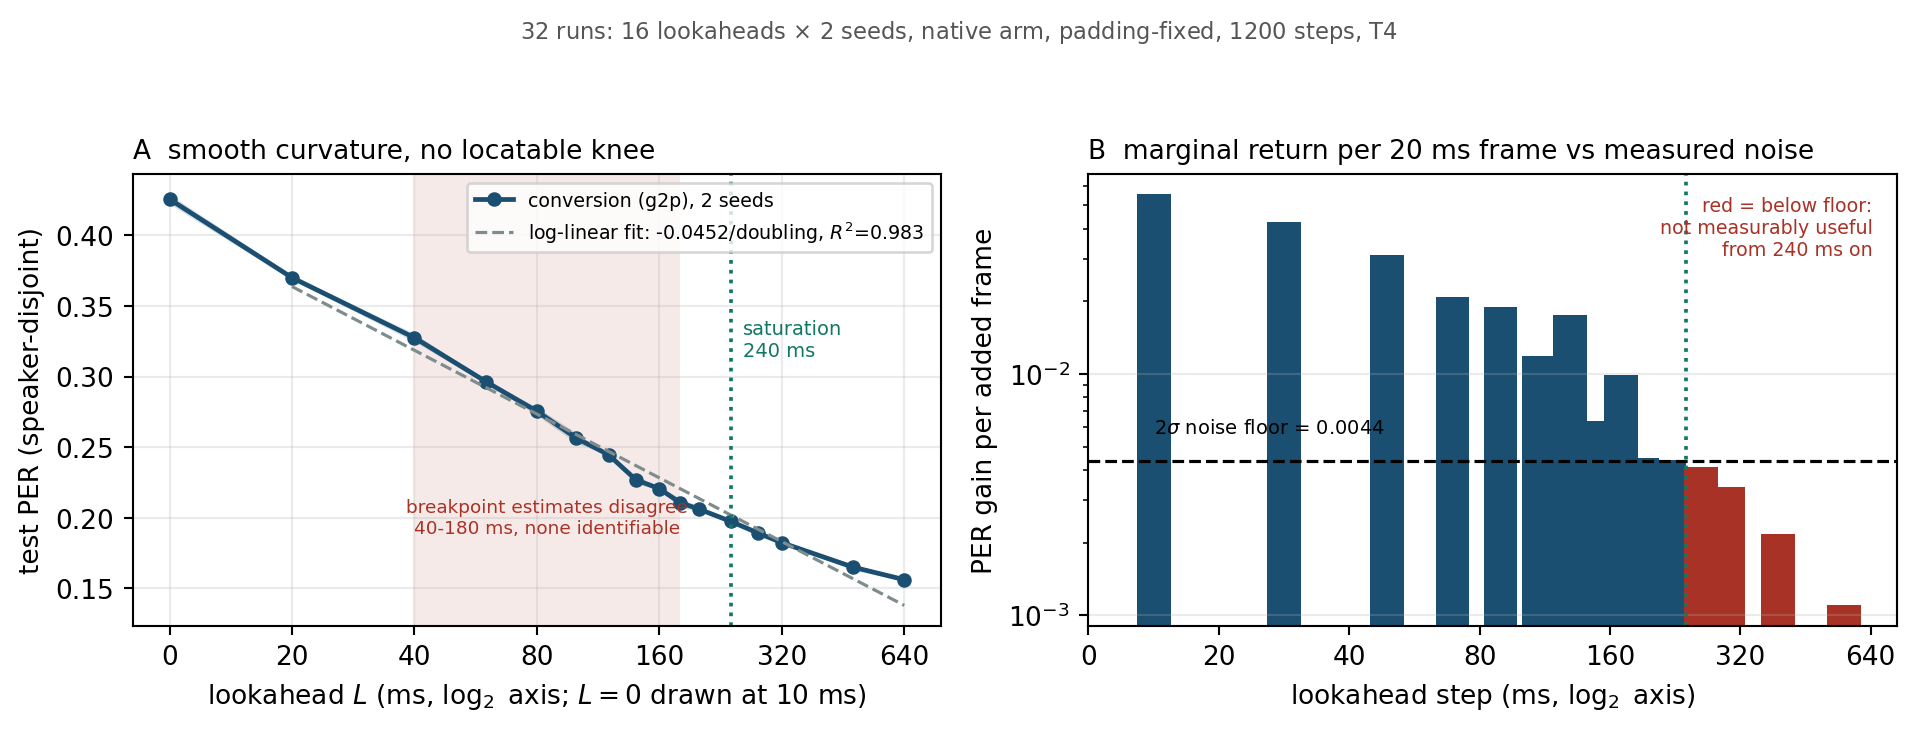
\includegraphics[width=\columnwidth]{../results/figures/fig_dense_no_knee.png}
\caption{Dense sweep, conversion arm, 16 lookaheads $\times$ 2 seeds.
\textbf{Left:} smooth curvature; the shaded band spans the breakpoint estimates
produced by three defensible treatments of $L{=}0$, none identifiable.
\textbf{Right:} marginal return per added 20\,ms frame against the measured
$2\sigma$ floor; red bars are below it.}
\label{fig:dense}
\end{figure}

Conversion-arm PER falls monotonically from $0.4256$ at $L{=}0$ to $0.1561$ at
$L{=}640$\,ms. Fitting $L\geq20$\,ms on $\log_2 L$ gives
\begin{equation}
\Delta\mathrm{PER} = -0.0452 \text{ per doubling},\quad R^2 = 0.983,
\end{equation}
over 15 points.

\textbf{There is curvature, and it is not localisable.} BIC prefers a
two-segment fit under all three axis treatments we tried
($\Delta\mathrm{BIC}=-22.2$, $-31.2$, $-36.8$), which by the usual
thresholds~\cite{kassraftery1995} is strong evidence. But the breakpoint lands
at 40, 180 and 180\,ms respectively, and every bootstrap 90\% interval spans
about three octaves. Sixteen points did not rescue a knee. The reason is
mechanical and worth stating: on a $\log_2(L{+}1)$ axis the $L{=}0
\rightarrow 20$\,ms gap is 4.39 units while every other gap is ${\approx}1.0$,
so a piecewise fit places a breakpoint just past that gap whatever the data
does.

\textbf{What we report instead} is the lookahead beyond which marginal return
falls below the measured floor. Per added 20\,ms frame, gains run
$+0.056$ (0$\rightarrow$20\,ms), $+0.021$ (60$\rightarrow$80),
$+0.0045$ (180$\rightarrow$200), and are below $0.0044$ for every step past
240\,ms. We therefore report \textbf{saturation at ${\approx}240$\,ms},
read as 200--280\,ms rather than a sharp value: the 140$\rightarrow$160 and
180$\rightarrow$200\,ms steps are already only 1.0--1.5$\times$ the floor.
Unlike a knee, this quantity depends only on the floor, not on an axis choice.

\begin{table}[t]
\centering\small
\caption{Conversion-arm PER against lookahead (mean of 2 seeds) and marginal
return per added 20\,ms frame, in units of the measured $2\sigma{=}0.0044$
floor. Below $1.0\times$ an additional frame is not measurably useful.}
\label{tab:dense}
\begin{tabular}{rrrr}
\toprule
$L$ (ms) & PER & gain/frame & $\times$ floor \\
\midrule
0   & 0.4256 & ---     & --- \\
20  & 0.3701 & 0.0556  & 12.7 \\
40  & 0.3275 & 0.0426  & 9.8 \\
60  & 0.2963 & 0.0312  & 7.2 \\
80  & 0.2754 & 0.0209  & 4.8 \\
100 & 0.2564 & 0.0190  & 4.4 \\
120 & 0.2446 & 0.0118  & 2.7 \\
140 & 0.2269 & 0.0176  & 4.0 \\
160 & 0.2206 & 0.0064  & 1.5 \\
180 & 0.2106 & 0.0099  & 2.3 \\
200 & 0.2062 & 0.0045  & 1.0 \\
240 & 0.1973 & 0.0044  & 1.0 \\
280 & 0.1891 & 0.0041  & \textbf{0.9} \\
320 & 0.1823 & 0.0034  & \textbf{0.8} \\
480 & 0.1649 & 0.0022  & \textbf{0.5} \\
640 & 0.1561 & 0.0011  & \textbf{0.3} \\
\bottomrule
\end{tabular}
\end{table}

\textbf{The cost of a 40\,ms budget.} PER at $L{=}40$\,ms is $0.3275$; at
240\,ms it is $0.1973$. A 40\,ms budget therefore forgoes \textbf{39.7\%} of
the achievable relative reduction, rising to 52.3\% against $L{=}640$\,ms.
``Current budgets are under-provisioned'' is thus supportable as
diminishing-returns geometry with a measurable saturation point --- not as a
knee.

\subsection{RQ2: manner class is the wrong axis}
\label{sec:rq2}

We pre-registered, before any of this data existed, that vowels and
approximants would break first (formant trajectories over 80--250\,ms) while
stops, fricatives, affricates and nasals would survive short lookahead (locally
determined gestures). Testing this on 295{,}785 reference phones, with each
substitution or deletion charged to the class of the \emph{reference} phone:

\begin{table}[t]
\centering\small
\caption{Relative error-rate reduction, $L{=}0\rightarrow640$\,ms. B =
pre-registered as breaking first, S = as surviving. The predicted grouping does
not order the data.}
\label{tab:h2}
\begin{tabular}{llrr}
\toprule
& class & rel.\ gain & ref.\ phones \\
\midrule
S & nasal        & 0.716 & 4\,020 \\
B & approximant  & 0.700 & 4\,575 \\
S & fricative    & 0.687 & 7\,659 \\
B & vowel (mono) & 0.673 & 13\,008 \\
B & vowel (diph) & 0.654 & 4\,824 \\
S & stop         & 0.615 & 7\,071 \\
S & affricate    & 0.525 & 1\,098 \\
\bottomrule
\end{tabular}
\end{table}

Group means differ in the predicted direction ($0.676$ vs $0.636$), but that is
the weakest available reading and three stronger checks fail. The effect size
is $0.66$: the between-group difference ($0.040$) is smaller than the pooled SD
across classes ($0.060$). The surviving group's \emph{internal} spread is
$0.190$ --- $4.7\times$ the between-group difference. And 5 of 12 pairwise
orderings are violated, with nasals out-gaining all three breaks-first classes.
By L1, only 3 of 6 support even the directional reading and the gain ratio
straddles unity ($0.92$ Chinese to $1.23$ Vietnamese).

\textbf{H2 is not supported.} The finding is not that lookahead fails to help
vowels --- every class improves 52--72\% relative, all above the floor. The
finding is that manner class does not predict which sounds need right context.

\textbf{Reweighting each error by what it costs acoustically does not rescue
it.} PER charges every error exactly 1.0, so a natural objection is that the
grouping is fine and PER is simply mis-weighting it: a substituted vowel and a
substituted stop cannot sound equally wrong. We tested that directly. Each
utterance's canonical phone string is synthesised with a fixed voice and
force-aligned to itself with an espeak-IPA CTC model, giving a time span per
reference phone; the hypothesis is synthesised, DTW-aligned to the reference,
and the spectral distortion inside each phone's own span is charged to that
phone's class. The measure is validated before it is used: phones the model got
wrong carry $1.72\times$ the distortion of phones it got right (86.8 vs 50.5),
so it does detect errors where they occur, and mean distortion falls
monotonically with lookahead (71.4 to 46.9, $-34\%$).

The verdict is unchanged (Table~\ref{tab:h2audio}). Acoustic weighting does move
in H2's favour --- effect size $0.607 \rightarrow 0.756$ and ordering violations
$4/12 \rightarrow 2/12$ against the sequence metric on the same utterances ---
but not far enough to clear the pre-registered threshold of $1.0$, and the
failure has the same shape as before: the ``survives'' group's internal spread
($0.120$) is $3.5\times$ the difference between the groups ($0.034$), and a
nasal again out-gains a diphthong. So ``PER mis-weights the classes'' is no
longer an available explanation for the sequence-level refutation.

\begin{table}[t]
\centering\small
\caption{H2 under acoustic weighting: relative reduction in per-phone
distortion, $L{=}0\rightarrow640$\,ms, 40 utterances, 1451 reference phones per
condition. B = pre-registered as breaking first, S = as surviving. The
sequence-metric column is computed on the same utterances, so the two differ
only in weighting.}
\label{tab:h2audio}
\begin{tabular}{llrrr}
\toprule
& class & acoustic & sequence & phones \\
\midrule
B & approximant  & 0.386 & 0.825 & 153 \\
B & vowel (mono) & 0.379 & 0.712 & 448 \\
S & nasal        & 0.376 & 0.784 & 128 \\
S & fricative    & 0.372 & 0.745 & 272 \\
B & vowel (diph) & 0.321 & 0.667 & 166 \\
S & stop         & 0.305 & 0.663 & 240 \\
S & affricate    & 0.257 & 0.526 & 44 \\
\midrule
\multicolumn{2}{l}{effect size (need $\geq1.0$)} & 0.756 & 0.607 & \\
\multicolumn{2}{l}{ordering violations} & 2/12 & 4/12 & \\
\bottomrule
\end{tabular}
\end{table}

One explanation does remain open, and it is not the one this test closes. Both
signals here are TTS renderings of phone strings, so the synthesiser produces
canonical formant trajectories for whatever string it is given. This measures
the cost of getting a phone's \emph{identity} wrong; it says nothing about a
wrong trajectory for a phone whose identity is right. That still needs real
converted audio against a native rendition (\S\ref{sec:remaining}). The sample
is also far smaller than the sequence-level test --- 1451 phones per condition
against 295{,}785 --- and is weighted accordingly.

\subsection{RQ3: conversion needs more lookahead than transcription}
\label{sec:rq3}

Identical architecture, capacity, data order, seed and step count; the two arms
differ only in the target tensor. Endpoint gain $L{=}0\rightarrow640$\,ms is
$-0.2695$ (63.2\% relative) for conversion against $-0.1893$ (42.8\%) for
accent-faithful transcription, a paired difference of $+0.0802$
($\mathrm{sd}=0.0035$, $t=39.7$).

\textbf{The dense grid replicates this, and sharpens it.} Running the full
16-lookahead $\times$ 2-seed sweep on the transcription arm as well puts both
arms on the same dense grid (Table~\ref{tab:h3dense}). The endpoint gains
reproduce the 7-point result almost exactly --- 63.3\% for conversion against
43.5\% for transcription, against 63.2\% and 42.8\% before --- on an
independent, denser sample. The exchange rates separate cleanly:
\begin{center}
conversion $-0.0452$ vs transcription $-0.0292$ PER per doubling,
\end{center}
$R^2 = 0.983$ and $0.984$ respectively, so \textbf{conversion buys
$\mathbf{1.55\times}$ as much per doubling of lookahead}.

The mechanism is visible in the gap rather than the levels. At $L{=}0$ the two
arms are nearly the same task ($0.4256$ vs $0.4427$, a gap of $0.0171$); by
$L{=}640$\,ms the gap is $0.0939$, \textbf{5.5$\times$ wider}. It widens in
13 of 15 adjacent steps, and the transcription arm is worse at 16 of 16
lookaheads, every one of them by more than the $0.0044$ noise floor. Lookahead,
not accuracy, is what separates them --- which is the claim H3 makes.

Two secondary points fall out. Both arms saturate at the same
${\approx}240$\,ms, and neither yields a locatable knee (breakpoints move to
$[40, 240, 160]$\,ms across axis treatments for transcription, against
$[40, 180, 180]$ for conversion), so \S\ref{sec:rq1}'s structural conclusion is
not an artefact of the conversion arm. And the transcription arm's own curve is
just as log-linear, so the shallower slope is a smaller effect of lookahead, not
a noisier measurement of the same one.

\begin{table}[t]
\centering\small
\caption{Both arms on the dense grid, mean of 2 seeds. The gap is the
transcription arm's PER minus the conversion arm's: near zero at $L{=}0$ and
widening monotonically with lookahead.}
\label{tab:h3dense}
\begin{tabular}{rrrr}
\toprule
$L$ (ms) & conversion & transcription & gap \\
\midrule
0   & 0.4256 & 0.4427 & $+$0.0171 \\
20  & 0.3700 & 0.3896 & $+$0.0196 \\
40  & 0.3275 & 0.3600 & $+$0.0325 \\
80  & 0.2754 & 0.3271 & $+$0.0517 \\
160 & 0.2206 & 0.2908 & $+$0.0702 \\
240 & 0.1973 & 0.2755 & $+$0.0782 \\
320 & 0.1823 & 0.2666 & $+$0.0843 \\
640 & 0.1561 & 0.2501 & $+$0.0939 \\
\midrule
\multicolumn{2}{l}{exchange rate (PER/doubling)} & & \\
\multicolumn{1}{r}{conversion} & $-0.0452$ & \multicolumn{2}{l}{$R^2=0.983$} \\
\multicolumn{1}{r}{transcription} & $-0.0292$ & \multicolumn{2}{l}{$R^2=0.984$} \\
\bottomrule
\end{tabular}
\end{table}

The claim is carried by the \emph{preference margin} --- PER against the other
arm's labels minus PER against its own --- which grows monotonically in 3/3
seeds for conversion ($+0.032$ at $L{=}0$ to $+0.099$ at 640\,ms; 18/18
adjacent step $\times$ seed comparisons positive) while the transcription
control is 0/3 monotone and drifts \emph{down} ($-0.0103$). Building the claim
on a difference rather than a level turned out to matter
(\S\ref{sec:lessons}).

\subsection{\tbuf{}: jitter measured, I/O not}
\label{sec:tbuf}

On the M4, two independent 30\,s duplex runs at 40\,ms blocks give a required
jitter buffer of $0.14$ and $0.08$\,ms, with p99 callback lateness
${\approx}0.06$\,ms, zero over/underruns and clock drift below
$1.3\times10^{-4}$\%. The jitter term is \textbf{negligible}.

The I/O term is \textbf{not measured}, and we report why rather than
substituting a number. An acoustic loopback failed on every attempt: the
captured level was invariant to output amplitude (peak $0.00505$ at amplitude
$0.50$ versus $0.00468$ at $0.95$), meaning the speaker contributes no
measurable energy to the microphone --- consistent with the operating system's
echo cancellation, which scales with its reference and therefore cannot be
defeated by a louder probe. The driver-reported figure is not a substitute: its
excess over the requested block is \emph{identically} 201.69\,ms at both 10 and
20\,ms blocks and then roughly doubles, i.e.\ it is queueing, not converter
delay.

\section{Three measurement failures}
\label{sec:lessons}

Each of the following produced plausible output before being caught. We report
them because each is a trap the next person will meet.

\textbf{A padding bug rewrote the curve's shape.} A masked block handed a
zero-padded hidden-state tensor to a depthwise convolution and feed-forward
that do not respect the key-padding mask. Fixing it was \emph{not} a constant
offset: the correction grows with lookahead, from $-0.014$\,PER at $L{=}0$ to
$-0.086$ at 320\,ms, a spread of $16.4\times$ the noise floor. The buggy curve
therefore \emph{understated} the benefit of lookahead, biasing the central
quantity of RQ1. A constant offset would have cancelled in every within-run
comparison; this did not. The preference margin (\S\ref{sec:rq3}) was
unaffected, because the bug moved both PERs together and the margin is a
difference.

\textbf{A breakpoint estimator returns a breakpoint whether or not one
exists.} $\Delta$BIC cannot distinguish ``there is a knee'' from ``piecewise
fits a curve better than a line''. Identifiability must be tested by perturbing
the x-axis and bootstrapping the location. Our synthetic check reproduces the
artefact exactly: on a curve that is log-linear for $L\geq20$ with $L{=}0$ off
the extrapolation, including $L{=}0$ yields $\Delta\mathrm{BIC}=-39$ and a
confident ``knee at 40\,ms''; dropping it yields $+5$ and no knee.

\textbf{An analysis that buckets unmatched symbols into ``other'' will produce
confident output on the wrong alphabet.} Our phoneme-class map was keyed on
ARPAbet; the sweep emits IPA. Applying one to the other sent 57\% of reference
tokens, including \emph{every vowel} and \textipa{/r/}, to ``other'' --- and
still printed per-class slopes, an H2 verdict and a by-L1 table. Assert
coverage; do not infer it from the absence of an error.

\section{Limitations}

Results are phone error rate, not perceived quality. No perceptual evaluation
was run, so nothing here supports a claim about naturalness or audible
accentedness; the saturation point says marginal \emph{PER} gain falls below
the noise floor, not that listeners stop noticing improvement. Training is
1200 steps, a comparison at fixed budget rather than to convergence. The dense
sweep uses two seeds per arm and contains no repeated cells, so its noise floor
is imported from the other sweep rather than re-measured.
\tbuf{}'s I/O term is unmeasured. The encoder is frozen throughout.

\section{Remaining work}
\label{sec:remaining}

Four items are outstanding, listed with what each would settle.

\textbf{(i) H2 on real converted audio.} The identity-error half of this is now
done (\S\ref{sec:rq2}): forced alignment charges each error its measured
acoustic cost, and the grouping still fails. What remains is the trajectory
half, which a TTS cannot answer because it renders canonical trajectories by
construction --- it needs a trained synthesis pipeline whose output can be
aligned against a native rendition. Note also that a VITS-class synthesiser is
globally coupled, so whole-utterance distortion cannot be charged to one phone;
the per-phone span from forced alignment is what makes the measurement local at
all (\texttt{docs/H2\_AUDIO\_DOMAIN\_BLOCKED.md}).

\textbf{(ii) \tbuf{} I/O on a platform without echo cancellation.} A wired
loopback, or measurement on the ARM64/Raspberry-Pi class this paper's
deployment argument is about, would close the one term of
Eq.~\ref{eq:decomp} that remains unmeasured.

\textbf{(iii) The hardware sweep beyond two architectures.} Compute is
currently characterised on Apple Silicon and ARM64 Linux. The embedded class is
projected, not measured.

\textbf{(iv) Perceptual evaluation.} Stimulus generation is implemented and the
inputs exist; only the rater study is unfunded. Every claim in this draft is
therefore scoped to PER, and the paper should not be submitted without either
running some form of perceptual check or stating this limitation as
prominently as \S8 does.

\section{Data and code availability}

Everything needed to reproduce every number is public. The harness, the
causality proof, the sweep configurations, the analysis scripts and their
self-tests, and the raw per-condition outputs are at
\url{https://github.com/Dipeshtripathi13/streaming-fac-lookahead}. This
includes the per-condition hypothesis dumps for both target arms, which are the
input to the phoneme-class and audio-domain analyses and cost a full sweep to
regenerate, and the host-identity JSON recorded alongside every timing.

Speech data is L2-ARCTIC~\cite{l2arctic2018}, obtained through the
\texttt{KoelLabs/L2Arctic} release (3599 phoneme-annotated utterances,
24 speakers, 6 L1s). That release is CC-BY-NC-4.0. The licence is
non-commercial, which is why no trained model weights are distributed; the
training code and configurations are released instead, and reproduce the
reported curves on a single mid-range GPU in a few hours.

\section{Acknowledgements}

This work used no external funding and no institutional compute. All GPU
results were obtained on free-tier Google Colab (Tesla T4); all CPU results on
consumer hardware. The author thanks the maintainers of L2-ARCTIC, WavLM,
sherpa-onnx and Piper, whose public releases made a single-author study of this
scope possible.

\todo{swap in the official Interspeech style file when the 2027 template is
published, and re-check the page limit: this draft is 4 pages of content plus
references, which meets the project's 4+2 target but not a 4+1 rule}

\section{Conclusion}

Lookahead buys accent-conversion quality at a stable exchange rate of
${\approx}0.045$ PER per doubling, with no knee to locate and measurable
returns out to ${\approx}240$\,ms --- six times the budget the current state of
the art uses, which forgoes about 40\% of the achievable reduction. Per-chunk
compute is flat across that range, so the trade-off is a modelling decision
rather than a hardware one. A pre-registered phoneme-class hypothesis was
refuted. We release the harness, the per-condition hypothesis dumps, and the
three measurement failures that had to be caught along the way.

\bibliographystyle{unsrt}
\bibliography{refs}

\end{document}
